% =====================================================================
% CHAPTER 2 -- Summary of: M. Beccaria et al., Scientific Reports, 2025 [Beccaria2025B]
% =====================================================================
\section*{CHAPTER 2. ROTATABLE BEAM-SCANNING CURVED SES}
\addcontentsline{toc}{section}{\numberline{}CHAPTER 2. ROTATABLE BEAM-SCANNING CURVED SES}
\setcounter{section}{2}
\setcounter{subsection}{0}
\setcounter{equation}{0}
\setcounter{theorem}{0}
\setcounter{figure}{0}
\setcounter{table}{0}

\subsection{Problem}
The curved SES of Chapter~1 is passive and has a fixed beam: rotating it around the pole adjusts the pointing direction only within about $\pm 3^\circ$~\cite{Beccaria2025B}. Reconfigurable intelligent surfaces (RISs) can scan the beam, but each cell needs a PIN diode, micro-electro-mechanical systems (MEMS) switch or liquid crystal, plus a control network, which makes them complex and expensive~\cite{Beccaria2025B}. In many outdoor scenarios the beam only needs to be re-pointed occasionally after installation. Beccaria \textit{et al.}~\cite{Beccaria2025B} point out that no passive, low-cost SES could scan its beam in this way.

\subsection{Contributions and Methodology}
Beccaria \textit{et al.}~\cite{Beccaria2025B} propose a passive curved SES that is concentric with the pole and steers its reflected beam when mechanically rotated around the pole by an angle $\alpha$ (Fig.~\ref{fig:ch2-principle}). According to the authors, this configuration is the first of its kind. A fixed metallic shutter exposes only a ``visible window'' of the skin to the BS, so each rotation angle illuminates a different part of the phase map. The design has three elements:
\begin{itemize}
    \item \textbf{Region-based phase map.} The skin is divided into five regions. Regions 1, 3 and 5 point the beam to one end, the centre and the other end of the scan range. Regions 2 and 4 are transitions designed with a bifocal approach: each takes the average of the phase delays of the central region and the adjacent end region. The paper~\cite{Beccaria2025B} states this rule in words; written as equations (our formalization), it reads
    \begin{equation}\label{eq:ch2-transition}
    \Delta\varphi^{(2)}_{ij} = \tfrac{1}{2}\bigl(\Delta\varphi^{(1)}_{ij} + \Delta\varphi^{(3)}_{ij}\bigr), \qquad
    \Delta\varphi^{(4)}_{ij} = \tfrac{1}{2}\bigl(\Delta\varphi^{(3)}_{ij} + \Delta\varphi^{(5)}_{ij}\bigr),
    \end{equation}
    where $\Delta\varphi^{(r)}_{ij}$ is the delay that cell $ij$ would need to point the beam in the direction assigned to region $r$.
    \item \textbf{Unit cell with integrated radome.} The cell is a square patch with a cross-shaped slot (arm width 0.4~mm, 0.2~mm from the patch edge) on a 0.508~mm grounded DiClad~527 substrate ($\varepsilon_r = 2.55$, $\tan\delta = 0.0022$). It is covered directly by a 1~mm Lexan radome ($\varepsilon_r = 2.8$, $\tan\delta = 0.01$), which also holds the substrate in its curved shape. The period is 3.6~mm, slightly below $\lambda_0/3$ at 27~GHz. Limiting the patch size to $W = 1.5$--$3.1$~mm avoids higher-order resonances. This gives a phase range slightly below $300^\circ$, with $|S_{11}| \geq -1$~dB for incidence angles from $0^\circ$ to $60^\circ$ (Floquet analysis in CST).
    \item \textbf{Design example.} The skin has $150 \times 40$ cells bent to a 175~mm radius, typical of light poles. It is designed at 27~GHz to scan $0^\circ$--$50^\circ$ in the horizontal plane. The central region ($63 \times 40$ cells) points at $\varphi_{\max} = 35^\circ$, and the visible window contains $84 \times 40$ cells.
\end{itemize}
Rotating the skin by $\alpha$ moves the visible window along the phase map. According to~\cite{Beccaria2025B}, the beam then turns by about twice the rotation angle, which we formalize as the approximate relation
\begin{equation}\label{eq:ch2-steering}
\varphi_{\max}(\alpha) \approx \varphi_{\max}(0) + 2\alpha .
\end{equation}
In a physical-optics (PO) check on a smaller skin ($99 \times 31$ cells, 150~mm radius), $\alpha = -5.35^\circ$ moved the beam from $35^\circ$ to about $23^\circ$.

\begin{figure}[!htbp]
    \centering
    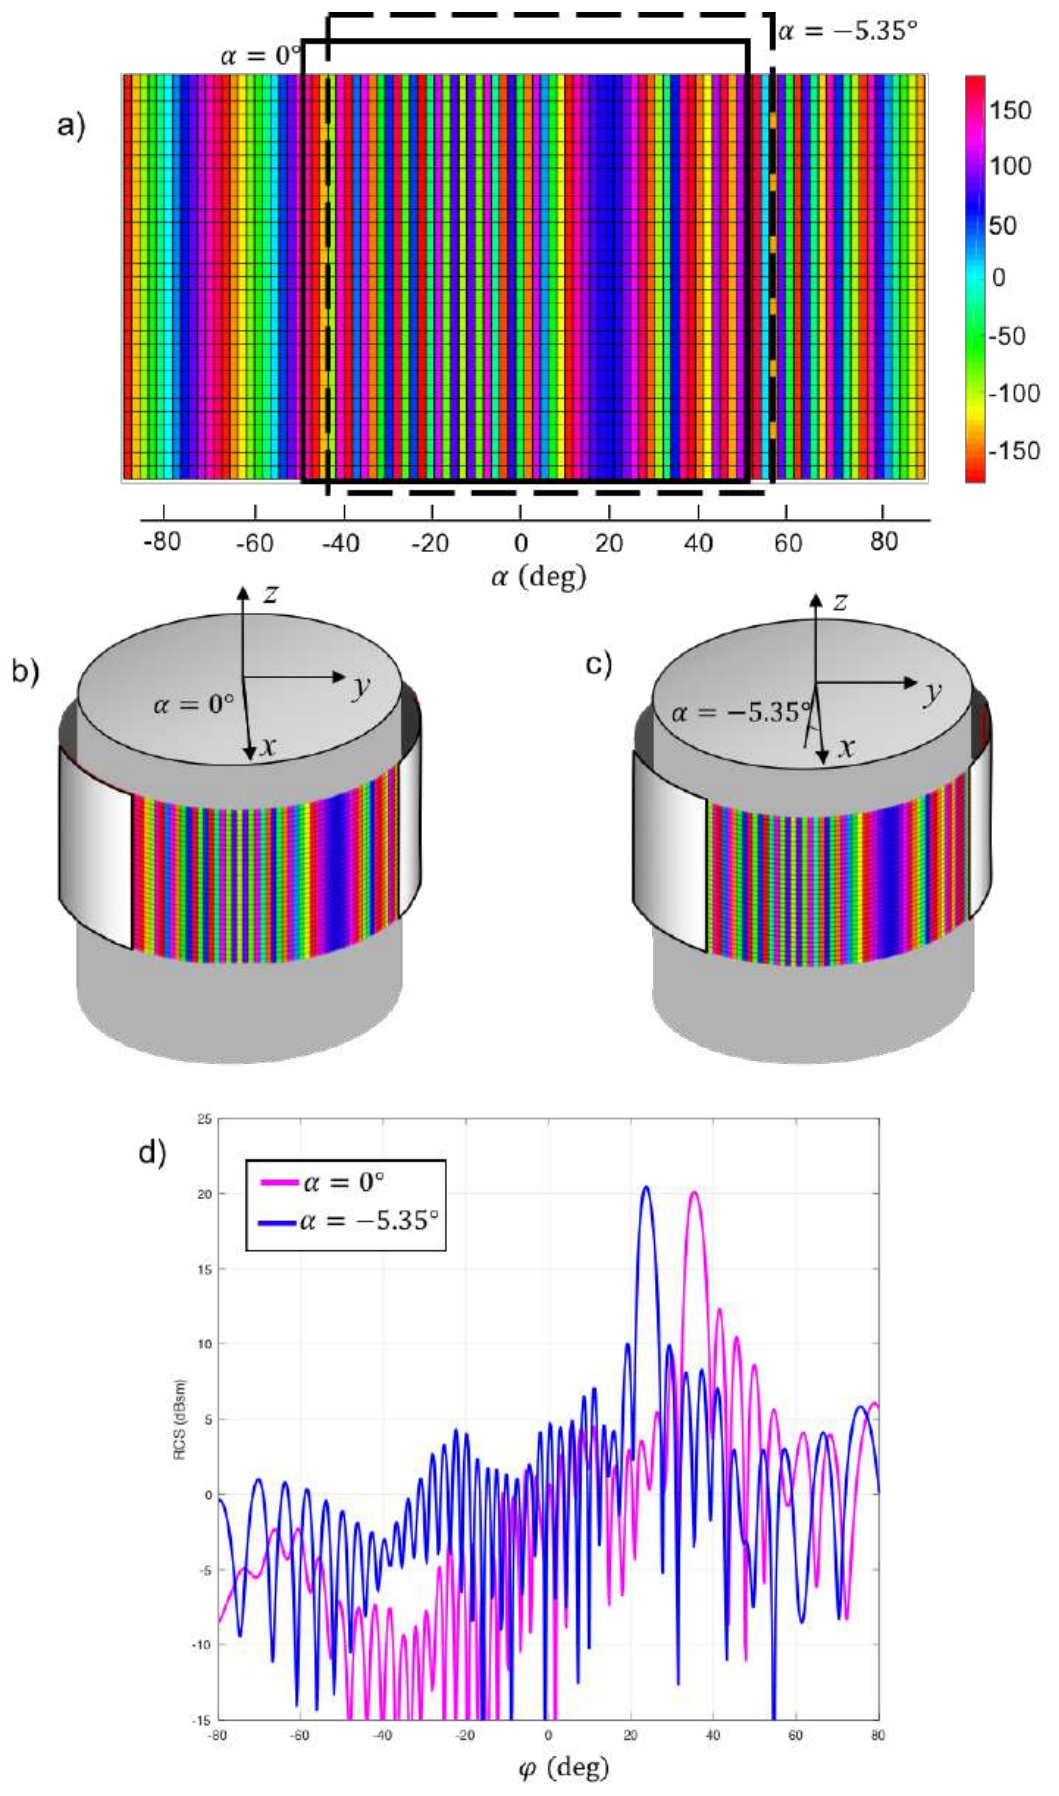
\includegraphics[height=0.5\textheight]{Images/ch2_beccaria_fig4.png}
    \caption[Working principle of the rotatable curved SES]{Working principle of the rotatable curved SES: (a) phase-delay map with the visible window for $\alpha = 0^\circ$ (solid box) and $\alpha = -5.35^\circ$ (dashed box); (b), (c) skin position for the two rotation angles; (d) horizontal-plane RCS computed with physical optics (adapted from~\cite{Beccaria2025B}).}
    \label{fig:ch2-principle}
\end{figure}

\subsection{Limitations of the Approach}
\begin{itemize}
    \item Only the part of the skin inside the visible window radiates, and its transition regions, defined by \eqref{eq:ch2-transition}, point elsewhere. For the same window, the main beam therefore uses less aperture than in a fixed-beam skin.
    \item Scanning is mechanical and limited to the horizontal plane. It requires a rotation mechanism (power is available on the pole) and cannot track users in real time as an RIS does.
    \item The unit cell does not reach a full $360^\circ$ phase cycle (below $300^\circ$).
    \item All results come from PO and CST simulations; no prototype was fabricated or measured.
\end{itemize}

\subsection{Results and Evaluation}
Table~\ref{tab:ch2-scan} gives the beam direction and the maximum RCS at 27~GHz for nine rotation angles~\cite{Beccaria2025B}. Rotating the skin from $\alpha = -21^\circ$ to $+7^\circ$ steers the beam from $-9.3^\circ$ to $50.6^\circ$, which covers the targeted $0^\circ$--$50^\circ$ sector. Each $3.5^\circ$ step moves the beam by $7.0^\circ$--$8.0^\circ$, in agreement with \eqref{eq:ch2-steering}.

The maximum RCS stays within about 1~dB up to $\varphi_{\max} \approx 43^\circ$ and drops by about 2.5~dB near $50^\circ$ (15.4~dBsm). Good patterns are harder to obtain at large pointing angles, and the scan range was deliberately not centred on the specular direction, a worst case. The worst side-lobe level, at $\alpha = 7^\circ$, is 8~dB below the maximum. At the band edges (26.5 and 27.5~GHz) the maximum RCS stays within $\pm 1.5$~dB, except at $\alpha = 7^\circ$, where it drops by about 3.5~dB at 26.5~GHz.

The authors also compare the skin with a fixed-beam curved SES of the same window size ($84 \times 40$ cells) pointing at $35^\circ$. The rotatable skin loses at most 1~dB of maximum RCS, in the lower part of the band. This is the cost of using one degree of freedom, the patch size, to serve several directions. The design is also robust. Errors of $\pm 1$~mm in the curvature radius, or $\pm 2\%$ in the permittivity of the substrate or the radome, leave the patterns almost unchanged. Patch-size errors larger than usual fabrication tolerances lower the maximum RCS by less than 0.5~dB.

\begin{table}[!htbp]
    \centering
    \caption[Beam direction and maximum RCS versus rotation angle]{Beam direction $\varphi_{\max}$ and maximum RCS at 27~GHz versus the rotation angle $\alpha$ of the curved SES (data from~\cite{Beccaria2025B}).}
    \label{tab:ch2-scan}
    \small
    \begin{tabular}{l*{9}{c}}
        \toprule
        $\alpha$ ($^\circ$) & $-21$ & $-17.5$ & $-14$ & $-10.5$ & $-7$ & $-3.5$ & $0$ & $+3.5$ & $+7$ \\
        \midrule
        $\varphi_{\max}$ ($^\circ$) & $-9.3$ & $-2.3$ & $5.0$ & $12.0$ & $19.6$ & $27.0$ & $35.0$ & $42.6$ & $50.6$ \\
        Max.\ RCS (dBsm) & 18.0 & 18.3 & 18.4 & 18.2 & 17.7 & 17.9 & 17.9 & 17.1 & 15.4 \\
        \bottomrule
    \end{tabular}
\end{table}

\subsection{Open Issues and Future Directions}
The authors suggest designing symmetric or wider scan ranges. They also suggest mounting a second SES on the free half of the pole, since one skin covers only $180^\circ$ of its perimeter~\cite{Beccaria2025B}. They further plan to make the design tolerant to different pole radii by adapting a curved-reflectarray technique that is valid for radii of $25\lambda$--$45\lambda$. The main missing step is experimental: fabricating the slotted-patch skin with its rotation mechanism and measuring it. Elevation scanning and the time needed to re-point the beam mechanically also remain open.
